% Options for packages loaded elsewhere
\PassOptionsToPackage{unicode}{hyperref}
\PassOptionsToPackage{hyphens}{url}
\PassOptionsToPackage{dvipsnames,svgnames,x11names}{xcolor}
%
\documentclass[
  letterpaper,
  DIV=11,
  numbers=noendperiod]{scrartcl}

\usepackage{amsmath,amssymb}
\usepackage{iftex}
\ifPDFTeX
  \usepackage[T1]{fontenc}
  \usepackage[utf8]{inputenc}
  \usepackage{textcomp} % provide euro and other symbols
\else % if luatex or xetex
  \usepackage{unicode-math}
  \defaultfontfeatures{Scale=MatchLowercase}
  \defaultfontfeatures[\rmfamily]{Ligatures=TeX,Scale=1}
\fi
\usepackage{lmodern}
\ifPDFTeX\else  
    % xetex/luatex font selection
\fi
% Use upquote if available, for straight quotes in verbatim environments
\IfFileExists{upquote.sty}{\usepackage{upquote}}{}
\IfFileExists{microtype.sty}{% use microtype if available
  \usepackage[]{microtype}
  \UseMicrotypeSet[protrusion]{basicmath} % disable protrusion for tt fonts
}{}
\makeatletter
\@ifundefined{KOMAClassName}{% if non-KOMA class
  \IfFileExists{parskip.sty}{%
    \usepackage{parskip}
  }{% else
    \setlength{\parindent}{0pt}
    \setlength{\parskip}{6pt plus 2pt minus 1pt}}
}{% if KOMA class
  \KOMAoptions{parskip=half}}
\makeatother
\usepackage{xcolor}
\setlength{\emergencystretch}{3em} % prevent overfull lines
\setcounter{secnumdepth}{5}
% Make \paragraph and \subparagraph free-standing
\ifx\paragraph\undefined\else
  \let\oldparagraph\paragraph
  \renewcommand{\paragraph}[1]{\oldparagraph{#1}\mbox{}}
\fi
\ifx\subparagraph\undefined\else
  \let\oldsubparagraph\subparagraph
  \renewcommand{\subparagraph}[1]{\oldsubparagraph{#1}\mbox{}}
\fi

\usepackage{color}
\usepackage{fancyvrb}
\newcommand{\VerbBar}{|}
\newcommand{\VERB}{\Verb[commandchars=\\\{\}]}
\DefineVerbatimEnvironment{Highlighting}{Verbatim}{commandchars=\\\{\}}
% Add ',fontsize=\small' for more characters per line
\newenvironment{Shaded}{}{}
\newcommand{\AlertTok}[1]{\textcolor[rgb]{0.58,0.85,0.30}{\textbf{\colorbox[rgb]{0.30,0.12,0.14}{#1}}}}
\newcommand{\AnnotationTok}[1]{\textcolor[rgb]{0.31,0.63,0.31}{#1}}
\newcommand{\AttributeTok}[1]{\textcolor[rgb]{0.65,0.15,0.64}{#1}}
\newcommand{\BaseNTok}[1]{\textcolor[rgb]{0.60,0.41,0.00}{#1}}
\newcommand{\BuiltInTok}[1]{\textcolor[rgb]{0.65,0.15,0.64}{#1}}
\newcommand{\CharTok}[1]{\textcolor[rgb]{0.31,0.63,0.31}{#1}}
\newcommand{\CommentTok}[1]{\textcolor[rgb]{0.63,0.63,0.65}{\textit{#1}}}
\newcommand{\CommentVarTok}[1]{\textcolor[rgb]{0.89,0.34,0.29}{\textit{#1}}}
\newcommand{\ConstantTok}[1]{\textcolor[rgb]{0.60,0.41,0.00}{#1}}
\newcommand{\ControlFlowTok}[1]{\textcolor[rgb]{0.65,0.15,0.64}{#1}}
\newcommand{\DataTypeTok}[1]{\textcolor[rgb]{0.65,0.15,0.64}{#1}}
\newcommand{\DecValTok}[1]{\textcolor[rgb]{0.60,0.41,0.00}{#1}}
\newcommand{\DocumentationTok}[1]{\textcolor[rgb]{0.89,0.34,0.29}{#1}}
\newcommand{\ErrorTok}[1]{\textcolor[rgb]{0.96,0.28,0.28}{\underline{#1}}}
\newcommand{\ExtensionTok}[1]{\textcolor[rgb]{0.25,0.47,0.95}{\textbf{#1}}}
\newcommand{\FloatTok}[1]{\textcolor[rgb]{0.60,0.41,0.00}{#1}}
\newcommand{\FunctionTok}[1]{\textcolor[rgb]{0.25,0.47,0.95}{#1}}
\newcommand{\ImportTok}[1]{\textcolor[rgb]{0.31,0.63,0.31}{#1}}
\newcommand{\InformationTok}[1]{\textcolor[rgb]{0.77,0.36,0.00}{#1}}
\newcommand{\KeywordTok}[1]{\textcolor[rgb]{0.65,0.15,0.64}{#1}}
\newcommand{\NormalTok}[1]{\textcolor[rgb]{0.22,0.23,0.26}{#1}}
\newcommand{\OperatorTok}[1]{\textcolor[rgb]{0.65,0.15,0.64}{#1}}
\newcommand{\OtherTok}[1]{\textcolor[rgb]{0.15,0.68,0.38}{#1}}
\newcommand{\PreprocessorTok}[1]{\textcolor[rgb]{0.65,0.15,0.64}{#1}}
\newcommand{\RegionMarkerTok}[1]{\textcolor[rgb]{0.16,0.50,0.73}{\colorbox[rgb]{0.08,0.19,0.26}{#1}}}
\newcommand{\SpecialCharTok}[1]{\textcolor[rgb]{0.00,0.52,0.74}{#1}}
\newcommand{\SpecialStringTok}[1]{\textcolor[rgb]{0.85,0.27,0.33}{#1}}
\newcommand{\StringTok}[1]{\textcolor[rgb]{0.31,0.63,0.31}{#1}}
\newcommand{\VariableTok}[1]{\textcolor[rgb]{0.89,0.34,0.29}{#1}}
\newcommand{\VerbatimStringTok}[1]{\textcolor[rgb]{0.85,0.27,0.33}{#1}}
\newcommand{\WarningTok}[1]{\textcolor[rgb]{0.85,0.27,0.33}{#1}}

\providecommand{\tightlist}{%
  \setlength{\itemsep}{0pt}\setlength{\parskip}{0pt}}\usepackage{longtable,booktabs,array}
\usepackage{calc} % for calculating minipage widths
% Correct order of tables after \paragraph or \subparagraph
\usepackage{etoolbox}
\makeatletter
\patchcmd\longtable{\par}{\if@noskipsec\mbox{}\fi\par}{}{}
\makeatother
% Allow footnotes in longtable head/foot
\IfFileExists{footnotehyper.sty}{\usepackage{footnotehyper}}{\usepackage{footnote}}
\makesavenoteenv{longtable}
\usepackage{graphicx}
\makeatletter
\def\maxwidth{\ifdim\Gin@nat@width>\linewidth\linewidth\else\Gin@nat@width\fi}
\def\maxheight{\ifdim\Gin@nat@height>\textheight\textheight\else\Gin@nat@height\fi}
\makeatother
% Scale images if necessary, so that they will not overflow the page
% margins by default, and it is still possible to overwrite the defaults
% using explicit options in \includegraphics[width, height, ...]{}
\setkeys{Gin}{width=\maxwidth,height=\maxheight,keepaspectratio}
% Set default figure placement to htbp
\makeatletter
\def\fps@figure{htbp}
\makeatother

\KOMAoption{captions}{tableheading}
\makeatletter
\@ifpackageloaded{caption}{}{\usepackage{caption}}
\AtBeginDocument{%
\ifdefined\contentsname
  \renewcommand*\contentsname{Table of contents}
\else
  \newcommand\contentsname{Table of contents}
\fi
\ifdefined\listfigurename
  \renewcommand*\listfigurename{List of Figures}
\else
  \newcommand\listfigurename{List of Figures}
\fi
\ifdefined\listtablename
  \renewcommand*\listtablename{List of Tables}
\else
  \newcommand\listtablename{List of Tables}
\fi
\ifdefined\figurename
  \renewcommand*\figurename{Figure}
\else
  \newcommand\figurename{Figure}
\fi
\ifdefined\tablename
  \renewcommand*\tablename{Table}
\else
  \newcommand\tablename{Table}
\fi
}
\@ifpackageloaded{float}{}{\usepackage{float}}
\floatstyle{ruled}
\@ifundefined{c@chapter}{\newfloat{codelisting}{h}{lop}}{\newfloat{codelisting}{h}{lop}[chapter]}
\floatname{codelisting}{Listing}
\newcommand*\listoflistings{\listof{codelisting}{List of Listings}}
\makeatother
\makeatletter
\makeatother
\makeatletter
\@ifpackageloaded{caption}{}{\usepackage{caption}}
\@ifpackageloaded{subcaption}{}{\usepackage{subcaption}}
\makeatother
\ifLuaTeX
  \usepackage{selnolig}  % disable illegal ligatures
\fi
\usepackage{bookmark}

\IfFileExists{xurl.sty}{\usepackage{xurl}}{} % add URL line breaks if available
\urlstyle{same} % disable monospaced font for URLs
\hypersetup{
  pdftitle={Descifrando patrones},
  colorlinks=true,
  linkcolor={blue},
  filecolor={Maroon},
  citecolor={Blue},
  urlcolor={Blue},
  pdfcreator={LaTeX via pandoc}}

\title{Descifrando patrones}
\usepackage{etoolbox}
\makeatletter
\providecommand{\subtitle}[1]{% add subtitle to \maketitle
  \apptocmd{\@title}{\par {\large #1 \par}}{}{}
}
\makeatother
\subtitle{Cómo utilizar los pronósticos para predecir el turismo en
México}
\author{}
\date{}

\begin{document}
\maketitle

\renewcommand*\contentsname{Table of contents}
{
\hypersetup{linkcolor=}
\setcounter{tocdepth}{3}
\tableofcontents
}
\begin{verbatim}
author: "Pablo Benavides Herrera"
format: 
  revealjs:
    transition: zoom
    logo: iteso.png
    footer: "Series de tiempo"
    scrollable: true
    theme: league
    self-contained: true
    execute:
      echo: false
\end{verbatim}

\section{¿Qué es una serie de
tiempo?}\label{quuxe9-es-una-serie-de-tiempo}

\begin{Shaded}
\begin{Highlighting}[]
\FunctionTok{library}\NormalTok{(pacman)}
\FunctionTok{p\_load}\NormalTok{(tidyverse, plotly, patchwork, timetk, modeltime, tidyquant, tsibble, feasts, fable, tsibbledata, fpp3, ggpubr, jpeg)}
\end{Highlighting}
\end{Shaded}

\subsection{}\label{section}

\begin{Shaded}
\begin{Highlighting}[]
\NormalTok{p }\OtherTok{\textless{}{-}}\NormalTok{ gapminder}\SpecialCharTok{::}\NormalTok{gapminder }\SpecialCharTok{|\textgreater{}} 
  \FunctionTok{ggplot}\NormalTok{(}\FunctionTok{aes}\NormalTok{(}\AttributeTok{x =}\NormalTok{ gdpPercap, }\AttributeTok{y =}\NormalTok{ lifeExp, }\AttributeTok{color =}\NormalTok{ country,}
                       \AttributeTok{size =}\NormalTok{ pop, }\AttributeTok{label =}\NormalTok{ country)) }\SpecialCharTok{+}
  \FunctionTok{geom\_point}\NormalTok{(}\FunctionTok{aes}\NormalTok{(}\AttributeTok{frame =}\NormalTok{ year)) }\SpecialCharTok{+} 
  \FunctionTok{scale\_x\_log10}\NormalTok{() }\SpecialCharTok{+} 
  \FunctionTok{ylab}\NormalTok{(}\StringTok{"Esperanza de vida (años)"}\NormalTok{) }\SpecialCharTok{+}
  \FunctionTok{xlab}\NormalTok{(}\StringTok{"PIB per cápita (USD, deflactado)"}\NormalTok{) }\SpecialCharTok{+}
  \FunctionTok{theme}\NormalTok{(}\AttributeTok{legend.position =} \StringTok{"none"}\NormalTok{)}
\end{Highlighting}
\end{Shaded}

\begin{verbatim}
Warning in geom_point(aes(frame = year)): Ignoring unknown aesthetics: frame
\end{verbatim}

\begin{Shaded}
\begin{Highlighting}[]
\FunctionTok{ggplotly}\NormalTok{(p)}
\end{Highlighting}
\end{Shaded}

\includegraphics{intro_files/figure-pdf/gapminder-1.pdf}

\subsection{}\label{section-1}

\subsection[\begin{center}

\end{center}
]{\texorpdfstring{\begin{center}
\protect
\includegraphics{fragua.png}
\end{center}
}{}}\label{section-2}

\begin{Shaded}
\begin{Highlighting}[]
\NormalTok{fragua }\OtherTok{\textless{}{-}} \FunctionTok{tq\_get}\NormalTok{(}\StringTok{"FRAGUAB.MX"}\NormalTok{, }\AttributeTok{from =} \StringTok{"2021{-}01{-}01"}\NormalTok{)}

\NormalTok{fragua }\SpecialCharTok{|\textgreater{}} 
  \FunctionTok{ggplot}\NormalTok{(}\FunctionTok{aes}\NormalTok{(}\AttributeTok{x =}\NormalTok{ date, }\AttributeTok{open =}\NormalTok{ open, }\AttributeTok{high =}\NormalTok{ high, }\AttributeTok{low =}\NormalTok{ low, }\AttributeTok{close =}\NormalTok{ close)) }\SpecialCharTok{+}
  \FunctionTok{geom\_barchart}\NormalTok{(}\AttributeTok{size =} \DecValTok{1}\NormalTok{) }\SpecialCharTok{+}
  \FunctionTok{geom\_bbands}\NormalTok{(}\AttributeTok{ma\_fun =}\NormalTok{ SMA, }\AttributeTok{sd =} \DecValTok{2}\NormalTok{, }\AttributeTok{n =} \DecValTok{20}\NormalTok{) }\SpecialCharTok{+}
  \FunctionTok{theme\_tq}\NormalTok{() }\SpecialCharTok{+}
  \FunctionTok{labs}\NormalTok{(}\AttributeTok{x =} \StringTok{""}\NormalTok{)}
\end{Highlighting}
\end{Shaded}

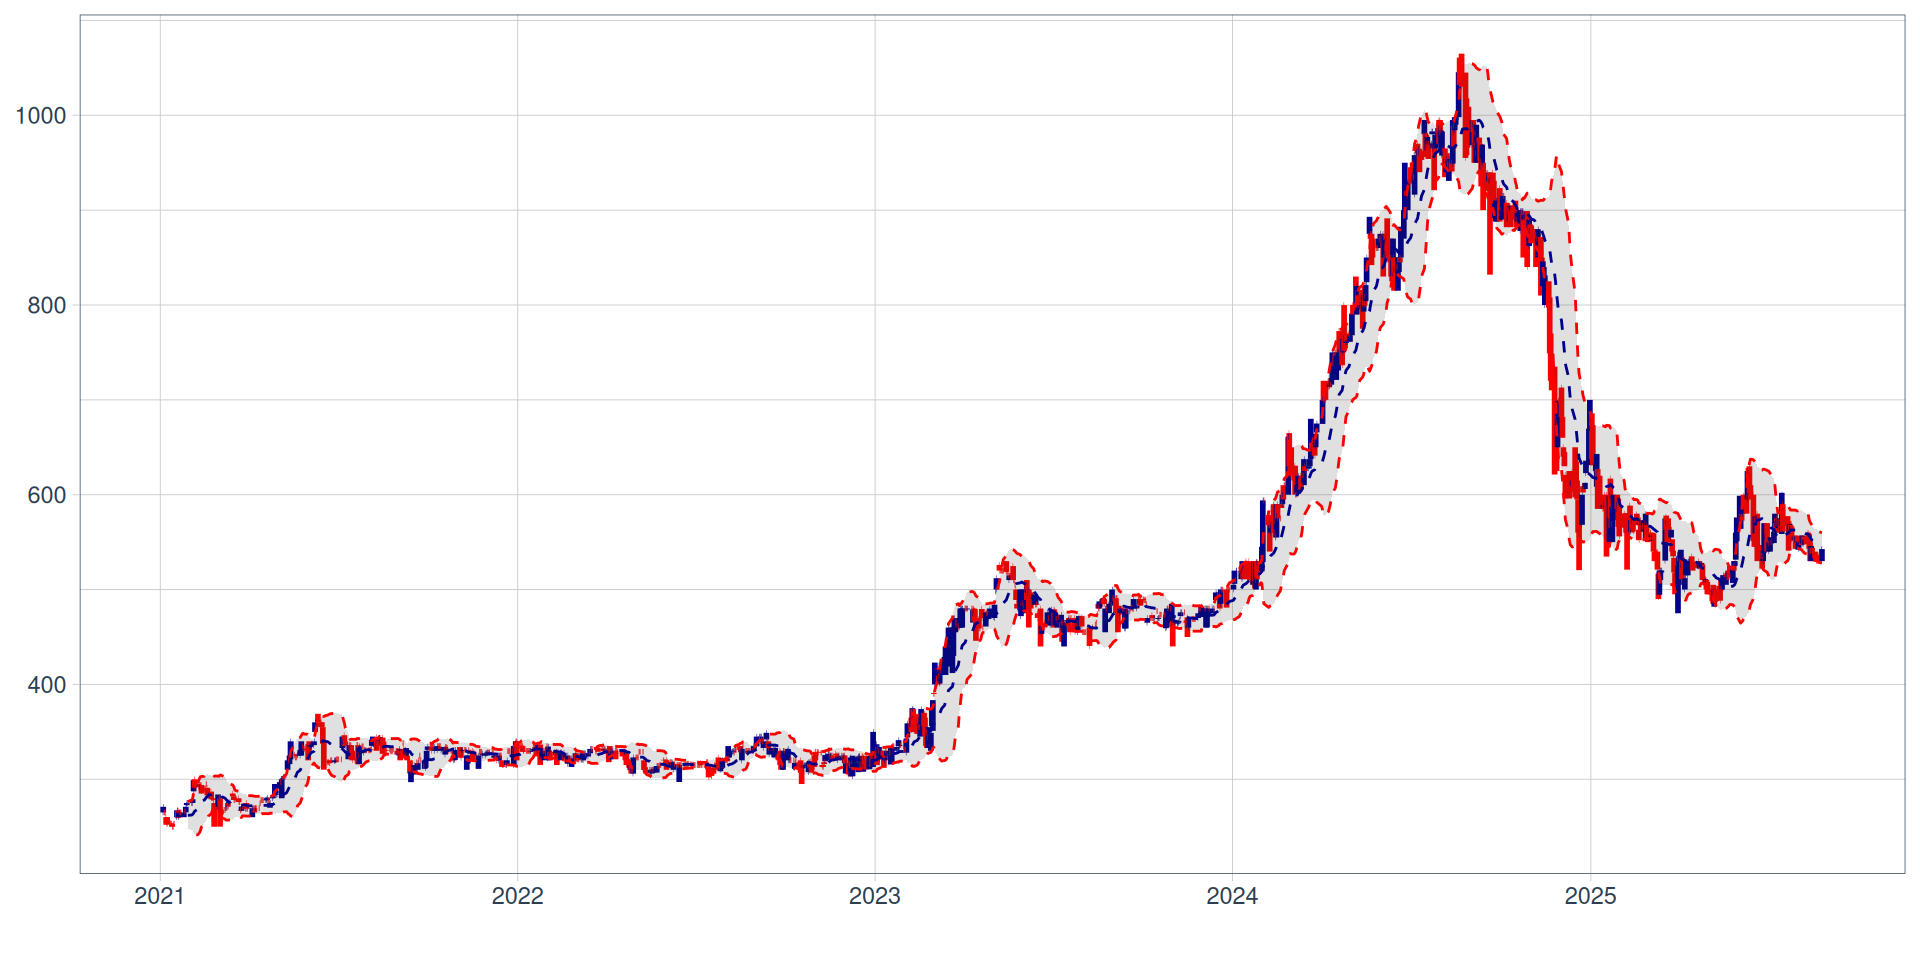
\includegraphics{intro_files/figure-pdf/fragua-1.pdf}

\subsection{¿Qué es un pronóstico?}\label{quuxe9-es-un-pronuxf3stico}

\subsection{}\label{section-3}

\subsection{}\label{section-4}

\subsection{}\label{section-5}

\subsection{Existen infinitas
posibilidades}\label{existen-infinitas-posibilidades}

\begin{Shaded}
\begin{Highlighting}[]
\NormalTok{google\_stock }\OtherTok{\textless{}{-}}\NormalTok{ tsibbledata}\SpecialCharTok{::}\NormalTok{gafa\_stock }\SpecialCharTok{\%\textgreater{}\%}
  \FunctionTok{filter}\NormalTok{(Symbol }\SpecialCharTok{==} \StringTok{"GOOG"}\NormalTok{) }\SpecialCharTok{\%\textgreater{}\%}
  \FunctionTok{mutate}\NormalTok{(}\AttributeTok{day =} \FunctionTok{row\_number}\NormalTok{()) }\SpecialCharTok{\%\textgreater{}\%}
\NormalTok{  tsibble}\SpecialCharTok{::}\FunctionTok{update\_tsibble}\NormalTok{(}\AttributeTok{index =}\NormalTok{ day, }\AttributeTok{regular =} \ConstantTok{TRUE}\NormalTok{)}

\CommentTok{\# Filter the year of interest}
\NormalTok{google\_2015 }\OtherTok{\textless{}{-}}\NormalTok{ google\_stock }\SpecialCharTok{\%\textgreater{}\%} \FunctionTok{filter}\NormalTok{(}\FunctionTok{year}\NormalTok{(Date) }\SpecialCharTok{==} \DecValTok{2015}\NormalTok{)}

\NormalTok{fit }\OtherTok{\textless{}{-}}\NormalTok{ google\_2015 }\SpecialCharTok{\%\textgreater{}\%}
  \FunctionTok{model}\NormalTok{(}\FunctionTok{NAIVE}\NormalTok{(Close))}

\NormalTok{sim }\OtherTok{\textless{}{-}}\NormalTok{ fit }\SpecialCharTok{\%\textgreater{}\%}  \FunctionTok{generate}\NormalTok{(}\AttributeTok{h =} \DecValTok{30}\NormalTok{, }\AttributeTok{times =} \DecValTok{10}\NormalTok{, }\AttributeTok{bootstrap =} \ConstantTok{TRUE}\NormalTok{, }\AttributeTok{seed =} \DecValTok{123}\NormalTok{)}

\NormalTok{p }\OtherTok{\textless{}{-}}\NormalTok{ google\_2015 }\SpecialCharTok{\%\textgreater{}\%}
  \FunctionTok{ggplot}\NormalTok{(}\FunctionTok{aes}\NormalTok{(}\AttributeTok{x =}\NormalTok{ day)) }\SpecialCharTok{+}
  \FunctionTok{geom\_line}\NormalTok{(}\FunctionTok{aes}\NormalTok{(}\AttributeTok{y =}\NormalTok{ Close), }\AttributeTok{size =} \DecValTok{1}\NormalTok{) }\SpecialCharTok{+}
  \FunctionTok{geom\_line}\NormalTok{(}\FunctionTok{aes}\NormalTok{(}\AttributeTok{y =}\NormalTok{ .sim, }\AttributeTok{colour =} \FunctionTok{as.factor}\NormalTok{(.rep)), }\AttributeTok{data =}\NormalTok{ sim, }\AttributeTok{size =} \DecValTok{1}\NormalTok{) }\SpecialCharTok{+}
  \FunctionTok{ggtitle}\NormalTok{(}\StringTok{"Google closing stock price"}\NormalTok{) }\SpecialCharTok{+}
  \FunctionTok{guides}\NormalTok{(}\AttributeTok{col =} \StringTok{"none"}\NormalTok{) }\SpecialCharTok{+}
  \FunctionTok{theme}\NormalTok{(}\AttributeTok{legend.position =} \StringTok{"none"}\NormalTok{)}

\FunctionTok{ggplotly}\NormalTok{(p, }\AttributeTok{dynamicTicks =} \ConstantTok{TRUE}\NormalTok{) }\SpecialCharTok{|\textgreater{}} \FunctionTok{rangeslider}\NormalTok{()}
\end{Highlighting}
\end{Shaded}

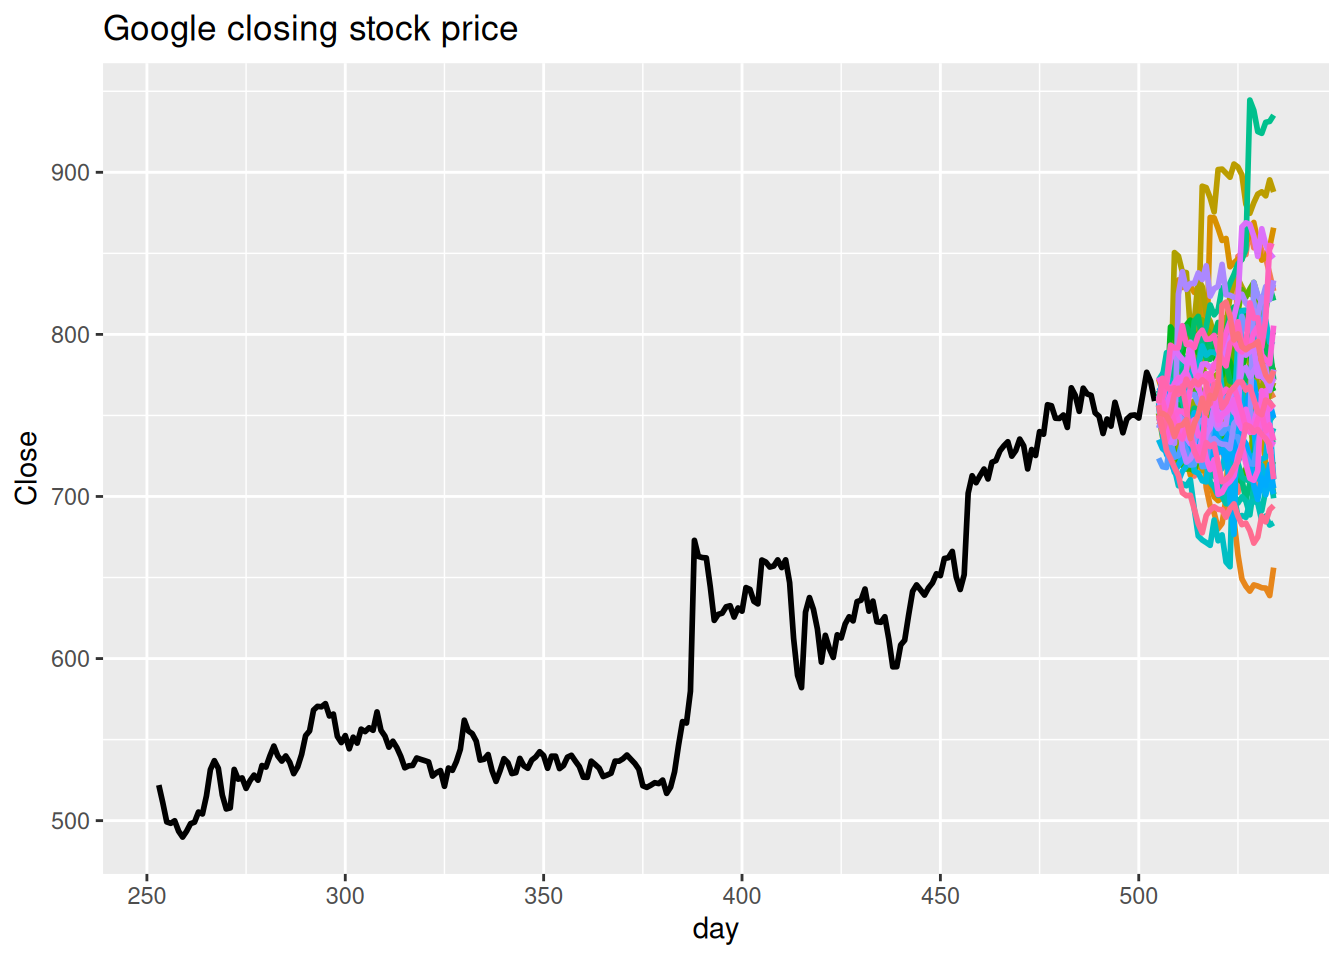
\includegraphics{intro_files/figure-pdf/google_2-1.pdf}

\subsection{Pronóstico de la producción de
cerveza}\label{pronuxf3stico-de-la-producciuxf3n-de-cerveza}

\begin{Shaded}
\begin{Highlighting}[]
\NormalTok{aus\_production }\SpecialCharTok{|\textgreater{}} 
  \FunctionTok{model}\NormalTok{(}\AttributeTok{arima =} \FunctionTok{ARIMA}\NormalTok{(Beer)) }\SpecialCharTok{|\textgreater{}} 
  \FunctionTok{forecast}\NormalTok{(}\AttributeTok{h =} \StringTok{"5 years"}\NormalTok{) }\SpecialCharTok{|\textgreater{}} 
  \FunctionTok{autoplot}\NormalTok{(aus\_production }\SpecialCharTok{|\textgreater{}} \FunctionTok{filter\_index}\NormalTok{(}\StringTok{"1990 Q1"} \SpecialCharTok{\textasciitilde{}}\NormalTok{ .), }\AttributeTok{size =} \DecValTok{1}\NormalTok{) }\SpecialCharTok{+}
  \FunctionTok{labs}\NormalTok{(}\AttributeTok{title =} \StringTok{"Producción de cerveza"}\NormalTok{,}
       \AttributeTok{x =} \StringTok{"Trimestre"}\NormalTok{,}
       \AttributeTok{y =} \StringTok{"Megalitros"}\NormalTok{)}
\end{Highlighting}
\end{Shaded}

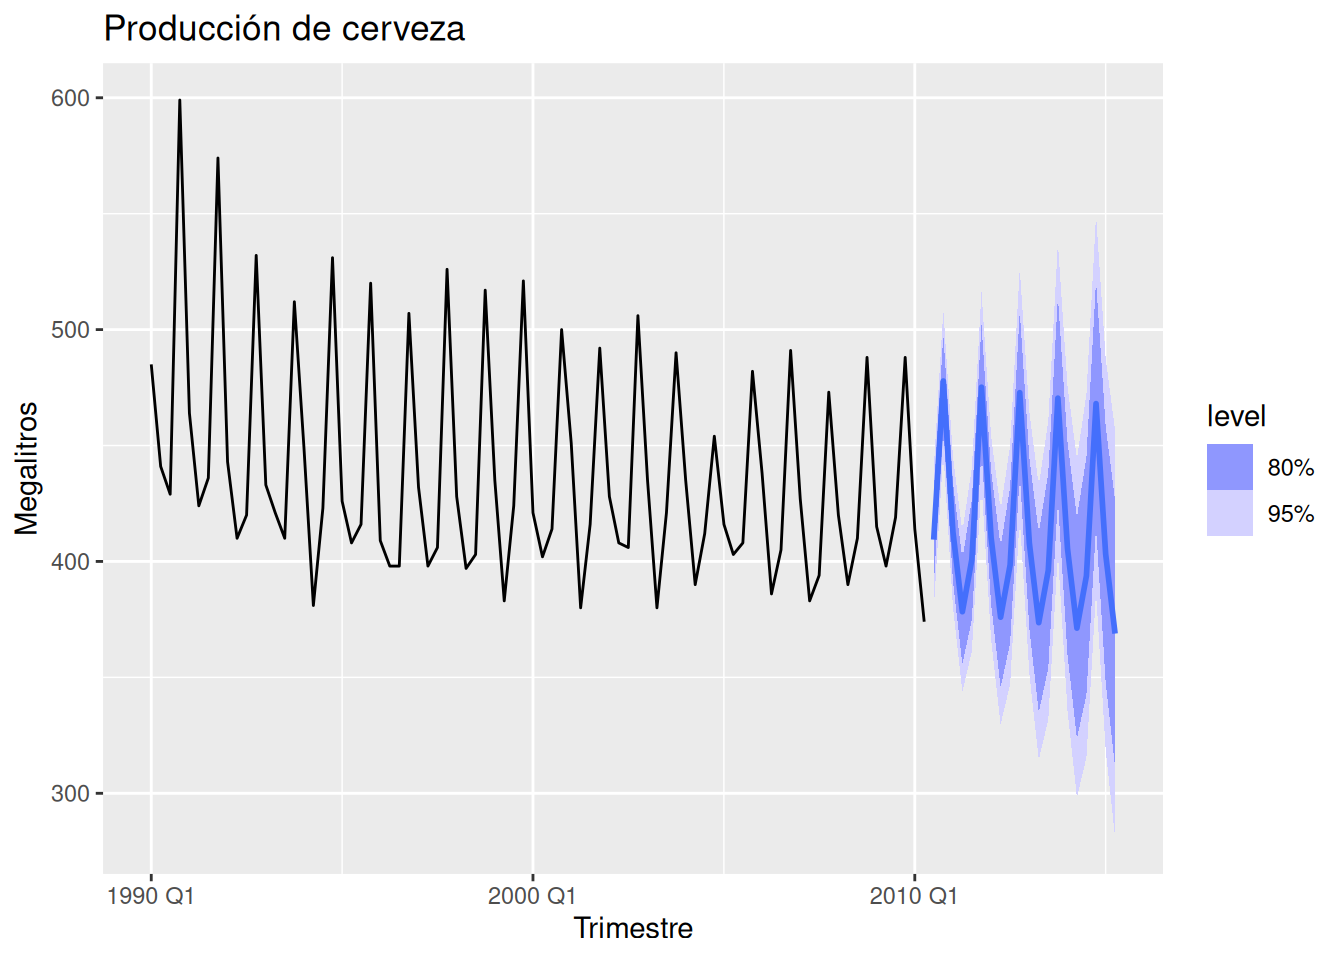
\includegraphics{intro_files/figure-pdf/beer-1.pdf}


\includegraphics{homer.png}

\subsection{Energía eléctrica}\label{energuxeda-eluxe9ctrica}

\begin{Shaded}
\begin{Highlighting}[]
\NormalTok{vic\_elec\_daily }\OtherTok{\textless{}{-}}\NormalTok{ vic\_elec }\SpecialCharTok{\%\textgreater{}\%}
  \CommentTok{\# filter(year(Time) == 2014) \%\textgreater{}\%}
  \FunctionTok{index\_by}\NormalTok{(}\AttributeTok{Date =} \FunctionTok{date}\NormalTok{(Time)) }\SpecialCharTok{\%\textgreater{}\%}
  \FunctionTok{summarise}\NormalTok{(}
    \AttributeTok{Demand =} \FunctionTok{sum}\NormalTok{(Demand)}\SpecialCharTok{/}\FloatTok{1e3}\NormalTok{,}
    \AttributeTok{Temperature =} \FunctionTok{max}\NormalTok{(Temperature),}
    \AttributeTok{Holiday =} \FunctionTok{any}\NormalTok{(Holiday)}
\NormalTok{  ) }\SpecialCharTok{\%\textgreater{}\%}
  \FunctionTok{mutate}\NormalTok{(}\AttributeTok{Day\_Type =} \FunctionTok{case\_when}\NormalTok{(}
\NormalTok{    Holiday }\SpecialCharTok{\textasciitilde{}} \StringTok{"Holiday"}\NormalTok{,}
    \FunctionTok{wday}\NormalTok{(Date) }\SpecialCharTok{\%in\%} \DecValTok{2}\SpecialCharTok{:}\DecValTok{6} \SpecialCharTok{\textasciitilde{}} \StringTok{"Weekday"}\NormalTok{,}
    \ConstantTok{TRUE} \SpecialCharTok{\textasciitilde{}} \StringTok{"Weekend"}
\NormalTok{  ))}

\NormalTok{vic\_elec\_daily }\SpecialCharTok{|\textgreater{}} 
  \FunctionTok{ggplot}\NormalTok{(}\FunctionTok{aes}\NormalTok{(}\AttributeTok{x =}\NormalTok{ Date, }\AttributeTok{y =}\NormalTok{ Demand)) }\SpecialCharTok{+}
  \FunctionTok{background\_image}\NormalTok{(}\FunctionTok{readJPEG}\NormalTok{(}\StringTok{"rick.jpg"}\NormalTok{)) }\SpecialCharTok{+}
  \FunctionTok{annotate}\NormalTok{(}\StringTok{"rect"}\NormalTok{, }\AttributeTok{xmin =} \FunctionTok{min}\NormalTok{(vic\_elec\_daily}\SpecialCharTok{$}\NormalTok{Date), }\AttributeTok{xmax =} \FunctionTok{max}\NormalTok{(vic\_elec\_daily}\SpecialCharTok{$}\NormalTok{Date), }\AttributeTok{ymin =} \SpecialCharTok{{-}}\ConstantTok{Inf}\NormalTok{, }\AttributeTok{ymax =} \ConstantTok{Inf}\NormalTok{, }\AttributeTok{fill =} \StringTok{"black"}\NormalTok{, }\AttributeTok{alpha =} \FloatTok{0.5}\NormalTok{) }\SpecialCharTok{+}
  \FunctionTok{geom\_line}\NormalTok{(}\AttributeTok{color =} \StringTok{"yellow2"}\NormalTok{) }\SpecialCharTok{+} \FunctionTok{theme\_dark}\NormalTok{()}
\end{Highlighting}
\end{Shaded}

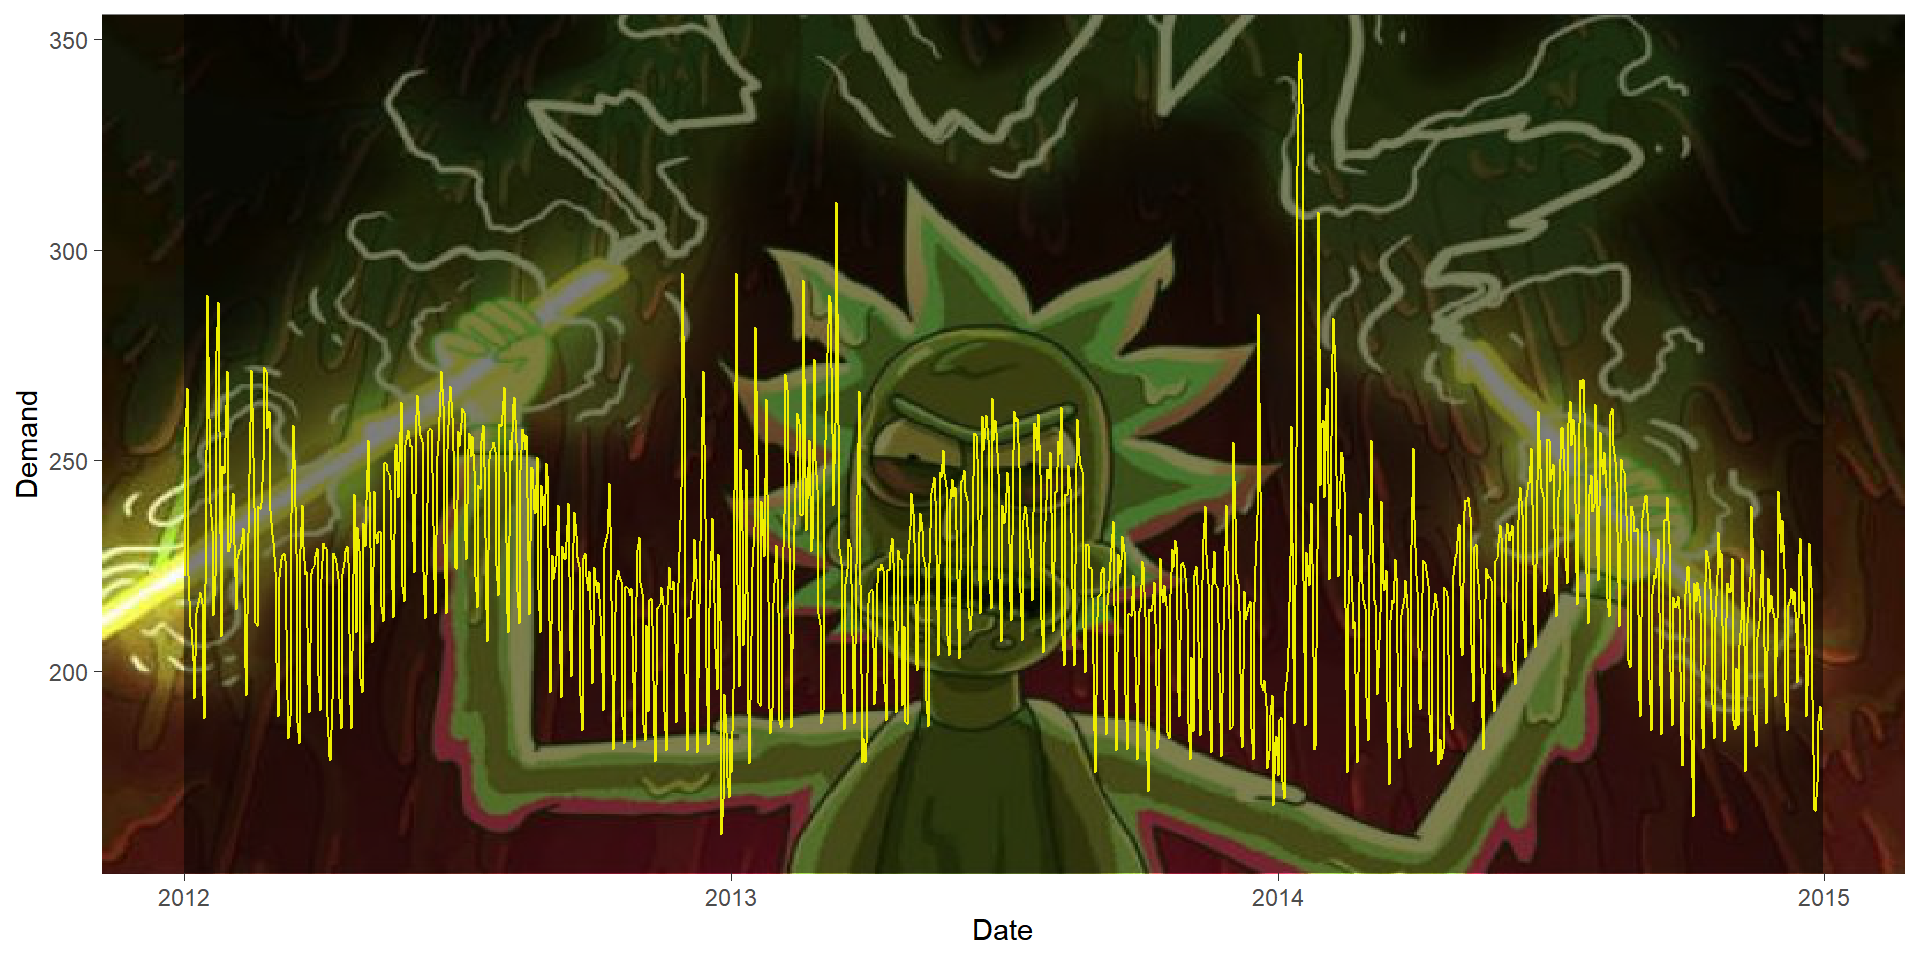
\includegraphics{intro_files/figure-pdf/energy-1.pdf}

\subsection{Demanda de energía
eléctrica}\label{demanda-de-energuxeda-eluxe9ctrica}

\begin{Shaded}
\begin{Highlighting}[]
\NormalTok{p }\OtherTok{\textless{}{-}}\NormalTok{ vic\_elec\_daily }\SpecialCharTok{|\textgreater{}} 
  \FunctionTok{ggplot}\NormalTok{(}\FunctionTok{aes}\NormalTok{(}\AttributeTok{x =}\NormalTok{ Date, }\AttributeTok{y =}\NormalTok{ Demand)) }\SpecialCharTok{+}
  \FunctionTok{geom\_line}\NormalTok{(}\AttributeTok{color =} \StringTok{"yellow2"}\NormalTok{, }\AttributeTok{size =} \DecValTok{1}\NormalTok{) }\SpecialCharTok{+}
  \FunctionTok{theme\_dark}\NormalTok{() }\SpecialCharTok{+}
  \FunctionTok{labs}\NormalTok{(}\AttributeTok{x =} \StringTok{"Fecha"}\NormalTok{, }\AttributeTok{y =} \StringTok{"Demanda"}\NormalTok{)}

\NormalTok{p}
\end{Highlighting}
\end{Shaded}

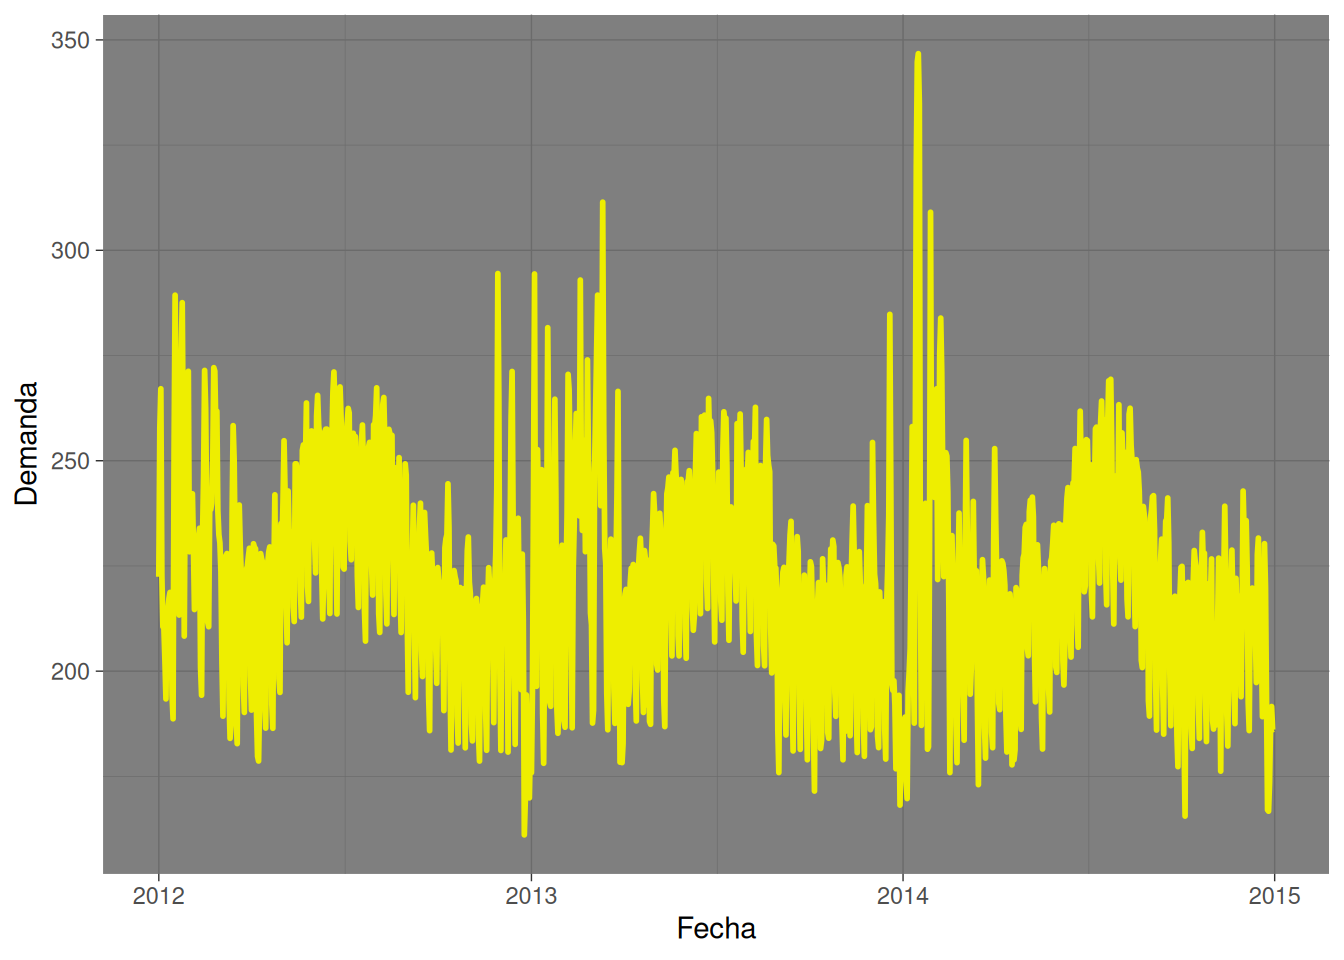
\includegraphics{intro_files/figure-pdf/energy_plotly-1.pdf}

\begin{Shaded}
\begin{Highlighting}[]
\CommentTok{\# ggplotly(p, dynamicTicks = TRUE) |\textgreater{} rangeslider()}
\end{Highlighting}
\end{Shaded}

\subsection{Empleo}\label{empleo}

\begin{Shaded}
\begin{Highlighting}[]
\NormalTok{us\_retail\_employment }\OtherTok{\textless{}{-}}\NormalTok{ us\_employment }\SpecialCharTok{\%\textgreater{}\%}
  \FunctionTok{filter}\NormalTok{(}\FunctionTok{year}\NormalTok{(Month) }\SpecialCharTok{\textgreater{}=} \DecValTok{1990}\NormalTok{, Title }\SpecialCharTok{==} \StringTok{"Retail Trade"}\NormalTok{)}

\NormalTok{p }\OtherTok{\textless{}{-}}\NormalTok{ us\_retail\_employment }\SpecialCharTok{|\textgreater{}} 
  \FunctionTok{ggplot}\NormalTok{(}\FunctionTok{aes}\NormalTok{(}\AttributeTok{x =}\NormalTok{ Month, }\AttributeTok{y =}\NormalTok{ Employed)) }\SpecialCharTok{+}
  \FunctionTok{geom\_line}\NormalTok{(}\AttributeTok{size =} \DecValTok{1}\NormalTok{, }\AttributeTok{color =} \StringTok{"purple"}\NormalTok{) }\SpecialCharTok{+}
  \FunctionTok{labs}\NormalTok{(}\AttributeTok{x =} \StringTok{"Mes"}\NormalTok{, }\AttributeTok{y =} \StringTok{"Empleados"}\NormalTok{) }\SpecialCharTok{+} 
  \FunctionTok{theme\_pubclean}\NormalTok{()}

\NormalTok{p}
\end{Highlighting}
\end{Shaded}

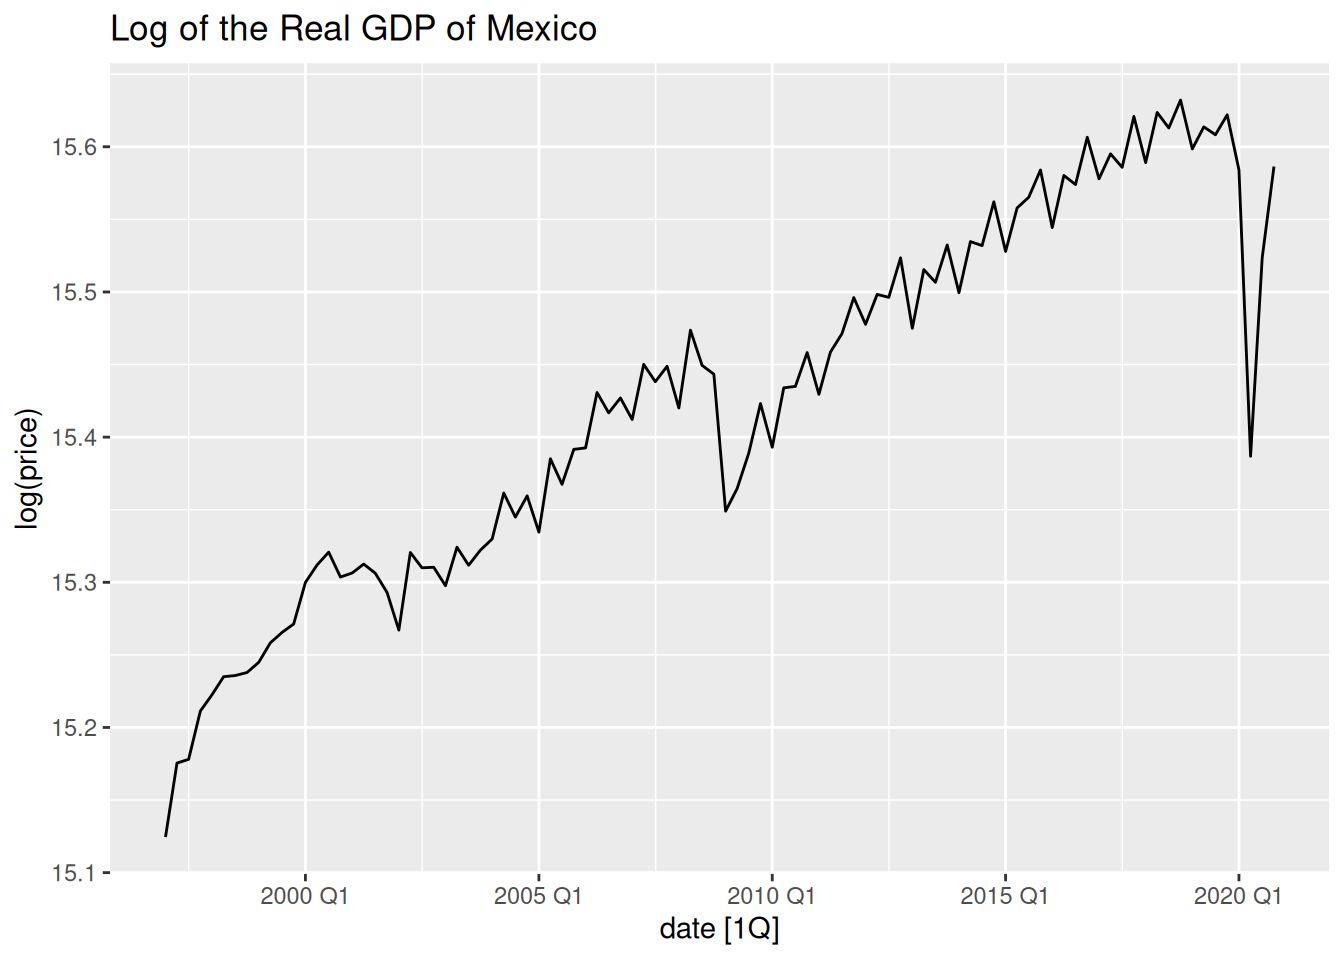
\includegraphics{intro_files/figure-pdf/unnamed-chunk-8-1.pdf}

\begin{Shaded}
\begin{Highlighting}[]
\CommentTok{\# ggplotly(p, dynamicTicks = TRUE) |\textgreater{} }
\CommentTok{\#   rangeslider()}
\end{Highlighting}
\end{Shaded}

\subsection{Empleo}\label{empleo-1}

\begin{Shaded}
\begin{Highlighting}[]
\NormalTok{us\_retail\_employment }\SpecialCharTok{|\textgreater{}} 
  \FunctionTok{model}\NormalTok{(}\AttributeTok{ets =} \FunctionTok{ARIMA}\NormalTok{(Employed)) }\SpecialCharTok{|\textgreater{}} 
  \FunctionTok{forecast}\NormalTok{(}\AttributeTok{h =} \StringTok{"6 years"}\NormalTok{) }\SpecialCharTok{|\textgreater{}} 
  \FunctionTok{autoplot}\NormalTok{(}\AttributeTok{color =} \StringTok{"purple"}\NormalTok{, }\AttributeTok{size =} \DecValTok{1}\NormalTok{) }\SpecialCharTok{+}
  \FunctionTok{autolayer}\NormalTok{(us\_retail\_employment, Employed, }\AttributeTok{color =} \StringTok{"purple"}\NormalTok{, }\AttributeTok{size =} \DecValTok{1}\NormalTok{) }\SpecialCharTok{+}
  \FunctionTok{theme\_pubclean}\NormalTok{() }\SpecialCharTok{+}
  \FunctionTok{labs}\NormalTok{(}\AttributeTok{x =} \StringTok{"Mes"}\NormalTok{, }\AttributeTok{y =} \StringTok{"Empleos"}\NormalTok{)}
\end{Highlighting}
\end{Shaded}

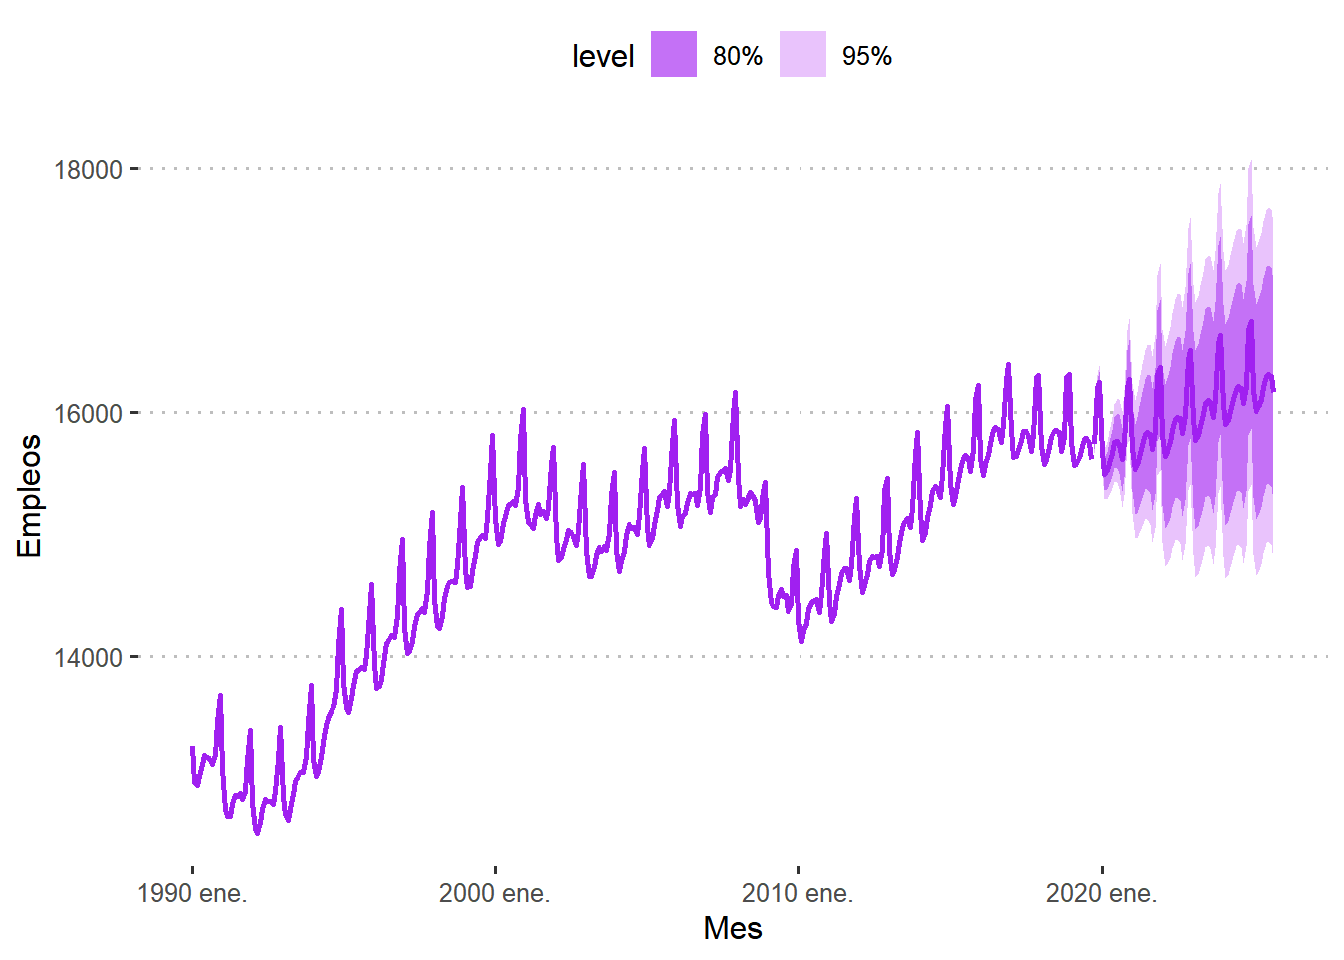
\includegraphics{intro_files/figure-pdf/unnamed-chunk-9-1.pdf}

\subsection{}\label{section-6}

\section{El turismo en México}\label{el-turismo-en-muxe9xico}

\subsection{}\label{section-7}

\begin{Shaded}
\begin{Highlighting}[]
\NormalTok{turismo }\OtherTok{\textless{}{-}}\NormalTok{ readxl}\SpecialCharTok{::}\FunctionTok{read\_excel}\NormalTok{(}\StringTok{"evi\_01.xlsx"}\NormalTok{, }\AttributeTok{skip =} \DecValTok{10}\NormalTok{, }\AttributeTok{col\_names =} \ConstantTok{TRUE}\NormalTok{) }\SpecialCharTok{|\textgreater{}} 
  \FunctionTok{slice}\NormalTok{(}\DecValTok{1}\SpecialCharTok{:}\DecValTok{6}\NormalTok{) }\SpecialCharTok{|\textgreater{}} 
\NormalTok{  janitor}\SpecialCharTok{::}\FunctionTok{remove\_empty}\NormalTok{()}
\end{Highlighting}
\end{Shaded}

\begin{verbatim}
value for "which" not specified, defaulting to c("rows", "cols")
\end{verbatim}

\begin{verbatim}
New names:
* `` -> `...1`
* `Entradas` -> `Entradas...2`
* `Salidas` -> `Salidas...3`
* `` -> `...4`
* `Entradas` -> `Entradas...5`
* `Salidas` -> `Salidas...6`
* `` -> `...7`
* `Entradas` -> `Entradas...8`
* `Salidas` -> `Salidas...9`
* `` -> `...10`
* `Entradas` -> `Entradas...11`
* `Salidas` -> `Salidas...12`
* `` -> `...13`
* `Entradas` -> `Entradas...14`
* `Salidas` -> `Salidas...15`
* `` -> `...16`
* `Entradas` -> `Entradas...17`
* `Salidas` -> `Salidas...18`
* `` -> `...19`
* `Entradas` -> `Entradas...20`
* `Salidas` -> `Salidas...21`
* `` -> `...22`
* `Entradas` -> `Entradas...23`
* `Salidas` -> `Salidas...24`
* `` -> `...25`
* `Entradas` -> `Entradas...26`
* `Salidas` -> `Salidas...27`
* `` -> `...28`
* `Entradas` -> `Entradas...29`
* `Salidas` -> `Salidas...30`
* `` -> `...31`
* `Entradas` -> `Entradas...32`
* `Salidas` -> `Salidas...33`
* `` -> `...34`
* `Entradas` -> `Entradas...35`
* `Salidas` -> `Salidas...36`
* `` -> `...37`
* `Entradas` -> `Entradas...38`
* `Salidas` -> `Salidas...39`
* `` -> `...40`
* `Entradas` -> `Entradas...41`
* `Salidas` -> `Salidas...42`
* `` -> `...43`
* `Entradas` -> `Entradas...44`
* `Salidas` -> `Salidas...45`
* `` -> `...46`
* `Entradas` -> `Entradas...47`
* `Salidas` -> `Salidas...48`
* `` -> `...49`
* `Entradas` -> `Entradas...50`
* `Salidas` -> `Salidas...51`
* `` -> `...52`
* `Entradas` -> `Entradas...53`
* `Salidas` -> `Salidas...54`
* `` -> `...55`
* `Entradas` -> `Entradas...56`
* `Salidas` -> `Salidas...57`
* `` -> `...58`
* `Entradas` -> `Entradas...59`
* `Salidas` -> `Salidas...60`
* `` -> `...61`
* `Entradas` -> `Entradas...62`
* `Salidas` -> `Salidas...63`
* `` -> `...64`
* `Entradas` -> `Entradas...65`
* `Salidas` -> `Salidas...66`
* `` -> `...67`
* `Entradas` -> `Entradas...68`
* `Salidas` -> `Salidas...69`
* `` -> `...70`
* `Entradas` -> `Entradas...71`
* `Salidas` -> `Salidas...72`
* `` -> `...73`
* `Entradas` -> `Entradas...74`
* `Salidas` -> `Salidas...75`
* `` -> `...76`
* `Entradas` -> `Entradas...77`
* `Salidas` -> `Salidas...78`
* `` -> `...79`
* `Entradas` -> `Entradas...80`
* `Salidas` -> `Salidas...81`
* `` -> `...82`
* `Entradas` -> `Entradas...83`
* `Salidas` -> `Salidas...84`
* `` -> `...85`
* `Entradas` -> `Entradas...86`
* `Salidas` -> `Salidas...87`
* `` -> `...88`
* `Entradas` -> `Entradas...89`
* `Salidas` -> `Salidas...90`
* `` -> `...91`
* `Entradas` -> `Entradas...92`
* `Salidas` -> `Salidas...93`
* `` -> `...94`
* `Entradas` -> `Entradas...95`
* `Salidas` -> `Salidas...96`
* `` -> `...97`
* `Entradas` -> `Entradas...98`
* `Salidas` -> `Salidas...99`
* `` -> `...100`
* `Entradas` -> `Entradas...101`
* `Salidas` -> `Salidas...102`
* `` -> `...103`
* `Entradas` -> `Entradas...104`
* `Salidas` -> `Salidas...105`
* `` -> `...106`
* `Entradas` -> `Entradas...107`
* `Salidas` -> `Salidas...108`
* `` -> `...109`
* `Entradas` -> `Entradas...110`
* `Salidas` -> `Salidas...111`
* `` -> `...112`
* `Entradas` -> `Entradas...113`
* `Salidas` -> `Salidas...114`
* `` -> `...115`
* `Entradas` -> `Entradas...116`
* `Salidas` -> `Salidas...117`
* `` -> `...118`
* `Entradas` -> `Entradas...119`
* `Salidas` -> `Salidas...120`
* `` -> `...121`
* `Entradas` -> `Entradas...122`
* `Salidas` -> `Salidas...123`
* `` -> `...124`
* `Entradas` -> `Entradas...125`
* `Salidas` -> `Salidas...126`
* `` -> `...127`
* `Entradas` -> `Entradas...128`
* `Salidas` -> `Salidas...129`
* `` -> `...130`
* `Entradas` -> `Entradas...131`
* `Salidas` -> `Salidas...132`
* `` -> `...133`
* `Entradas` -> `Entradas...134`
* `Salidas` -> `Salidas...135`
* `` -> `...136`
* `Entradas` -> `Entradas...137`
* `Salidas` -> `Salidas...138`
* `` -> `...139`
* `Entradas` -> `Entradas...140`
* `Salidas` -> `Salidas...141`
* `` -> `...142`
* `Entradas` -> `Entradas...143`
* `Salidas` -> `Salidas...144`
* `` -> `...145`
* `Entradas` -> `Entradas...146`
* `Salidas` -> `Salidas...147`
* `` -> `...148`
* `Entradas` -> `Entradas...149`
* `Salidas` -> `Salidas...150`
* `` -> `...151`
* `Entradas` -> `Entradas...152`
* `Salidas` -> `Salidas...153`
* `` -> `...154`
* `Entradas` -> `Entradas...155`
* `Salidas` -> `Salidas...156`
* `` -> `...157`
* `Entradas` -> `Entradas...158`
* `Salidas` -> `Salidas...159`
* `` -> `...160`
* `Entradas` -> `Entradas...161`
* `Salidas` -> `Salidas...162`
* `` -> `...163`
* `Entradas` -> `Entradas...164`
* `Salidas` -> `Salidas...165`
* `` -> `...166`
* `Entradas` -> `Entradas...167`
* `Salidas` -> `Salidas...168`
* `` -> `...169`
* `Entradas` -> `Entradas...170`
* `Salidas` -> `Salidas...171`
\end{verbatim}

\begin{Shaded}
\begin{Highlighting}[]
\NormalTok{turismo\_long }\OtherTok{\textless{}{-}}\NormalTok{ turismo }\SpecialCharTok{|\textgreater{}} 
  \FunctionTok{rename}\NormalTok{(}\AttributeTok{tipo\_turismo =}\NormalTok{ ...}\DecValTok{1}\NormalTok{) }\SpecialCharTok{|\textgreater{}} 
  \FunctionTok{select}\NormalTok{(tipo\_turismo, }\FunctionTok{starts\_with}\NormalTok{(}\StringTok{"Entradas"}\NormalTok{)) }\SpecialCharTok{|\textgreater{}} 
  \FunctionTok{pivot\_longer}\NormalTok{(}\AttributeTok{cols =} \SpecialCharTok{{-}}\NormalTok{ tipo\_turismo) }\SpecialCharTok{|\textgreater{}} 
  \FunctionTok{select}\NormalTok{(}\SpecialCharTok{{-}}\NormalTok{name) }\SpecialCharTok{|\textgreater{}} 
  \FunctionTok{group\_by}\NormalTok{(tipo\_turismo) }\SpecialCharTok{|\textgreater{}} 
  \FunctionTok{mutate}\NormalTok{(}\AttributeTok{date =} \FunctionTok{seq}\NormalTok{(}\FunctionTok{as.Date}\NormalTok{(}\StringTok{"2018{-}08{-}01"}\NormalTok{), }\FunctionTok{as.Date}\NormalTok{(}\StringTok{"2023{-}04{-}01"}\NormalTok{), }\AttributeTok{by =} \StringTok{"month"}\NormalTok{)) }\SpecialCharTok{|\textgreater{}} 
  \FunctionTok{relocate}\NormalTok{(date) }\SpecialCharTok{|\textgreater{}} 
  \FunctionTok{ungroup}\NormalTok{()}
\end{Highlighting}
\end{Shaded}

\begin{Shaded}
\begin{Highlighting}[]
\NormalTok{turismo\_tsbl }\OtherTok{\textless{}{-}}\NormalTok{ turismo\_long }\SpecialCharTok{|\textgreater{}} 
  \FunctionTok{mutate}\NormalTok{(}\AttributeTok{date =} \FunctionTok{yearmonth}\NormalTok{(date)) }\SpecialCharTok{|\textgreater{}} 
  \FunctionTok{as\_tsibble}\NormalTok{(}\AttributeTok{index =}\NormalTok{ date, }\AttributeTok{key =}\NormalTok{ tipo\_turismo)}
\end{Highlighting}
\end{Shaded}

\begin{Shaded}
\begin{Highlighting}[]
\NormalTok{p }\OtherTok{\textless{}{-}}\NormalTok{ turismo\_tsbl }\SpecialCharTok{|\textgreater{}} 
  \FunctionTok{autoplot}\NormalTok{(value) }\SpecialCharTok{+}
  \FunctionTok{facet\_wrap}\NormalTok{(}\SpecialCharTok{\textasciitilde{}} \FunctionTok{factor}\NormalTok{(tipo\_turismo, }\AttributeTok{levels =} \FunctionTok{c}\NormalTok{(}\StringTok{"Turistas de internación"}\NormalTok{, }\StringTok{"Vía aérea"}\NormalTok{, }\StringTok{"Vía terrestre"}\NormalTok{, }
                                               \StringTok{"Turistas fronterizos"}\NormalTok{, }\StringTok{"En automóviles"}\NormalTok{, }\StringTok{"Peatones"}\NormalTok{)), }\AttributeTok{ncol =} \DecValTok{3}\NormalTok{) }\SpecialCharTok{+}
  \FunctionTok{theme}\NormalTok{(}\AttributeTok{legend.position =} \StringTok{"none"}\NormalTok{)}

\NormalTok{p}
\end{Highlighting}
\end{Shaded}

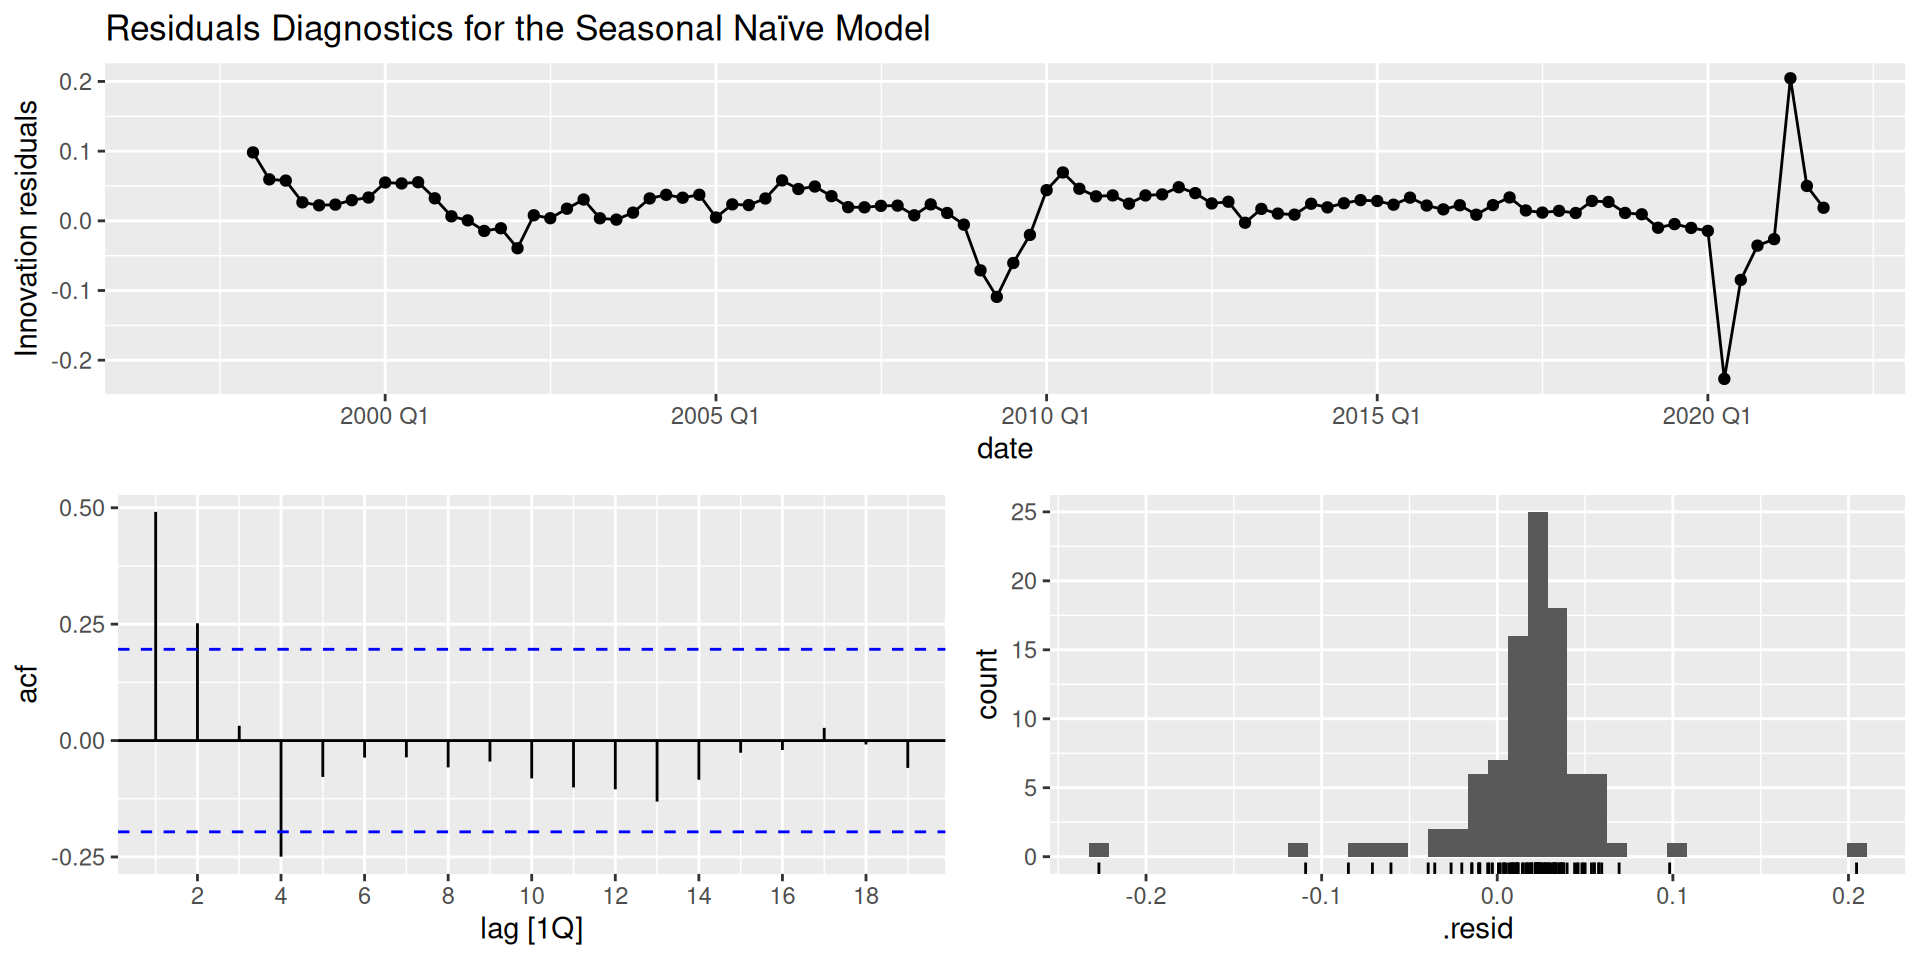
\includegraphics{intro_files/figure-pdf/unnamed-chunk-13-1.pdf}

\begin{Shaded}
\begin{Highlighting}[]
\CommentTok{\# ggplotly(p)}
\end{Highlighting}
\end{Shaded}

\begin{Shaded}
\begin{Highlighting}[]
\CommentTok{\# turismo\_long |\textgreater{} }
\CommentTok{\#   filter(tipo\_turismo == "Turistas de internación") |\textgreater{} }
\CommentTok{\#   select({-}tipo\_turismo) |\textgreater{} }
\CommentTok{\#   write\_csv("turismo.csv")}

\NormalTok{turismo\_tsbl }\SpecialCharTok{|\textgreater{}} 
  \FunctionTok{filter}\NormalTok{(tipo\_turismo }\SpecialCharTok{==} \StringTok{"Turistas de internación"}\NormalTok{) }\SpecialCharTok{|\textgreater{}} 
  \CommentTok{\# filter(tipo\_turismo \%in\% c("Vía aérea", "Vía terrestre")) |\textgreater{} }
  \FunctionTok{model}\NormalTok{(}
    \AttributeTok{arima =} \FunctionTok{ETS}\NormalTok{(value)}
\NormalTok{  ) }\SpecialCharTok{|\textgreater{}} 
  \FunctionTok{forecast}\NormalTok{(}\AttributeTok{h =} \StringTok{"3 years"}\NormalTok{) }\SpecialCharTok{|\textgreater{}} 
  \FunctionTok{autoplot}\NormalTok{(turismo\_tsbl)}
\end{Highlighting}
\end{Shaded}

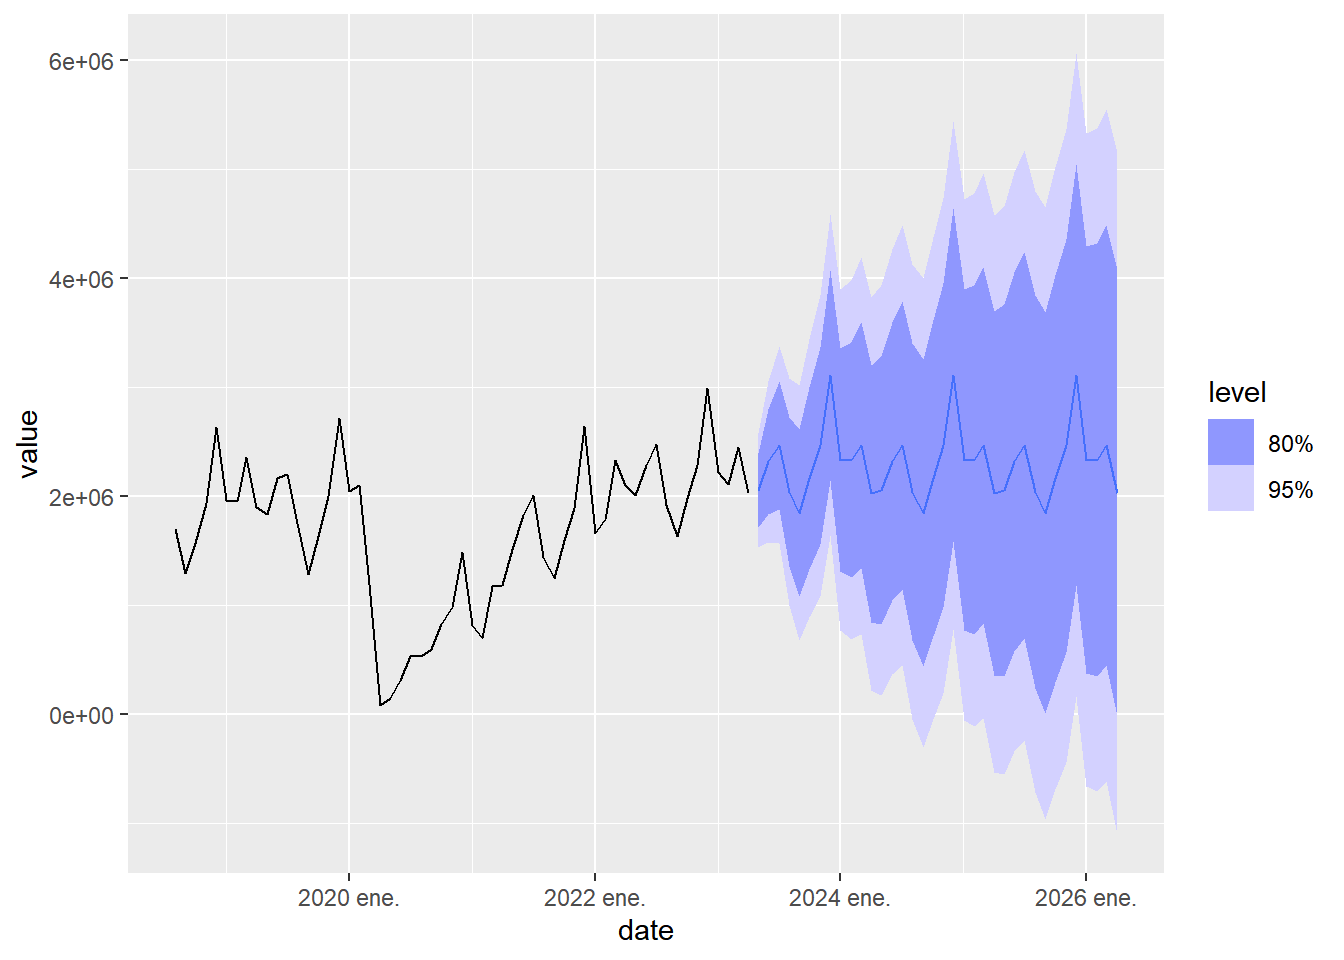
\includegraphics{intro_files/figure-pdf/unnamed-chunk-14-1.pdf}



\end{document}
